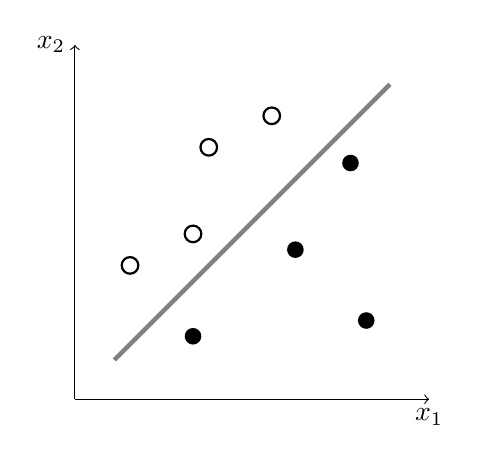
\begin{tikzpicture}[scale=1]
  % osi
  \draw[->] (0,0) -- (4.5,0) node[below] {$x_1$};
  \draw[->] (0,0) -- (0,4.5) node[left] {$x_2$};

  % trieda 1 - štvorčeky
  \foreach \x/\y in {1.7/3.2, 2.5/3.6, 0.7/1.7, 1.5/2.1}
    \draw[thick] (\x,\y) circle (3 pt);

  % trieda 2 - plné štvorce
  \foreach \x/\y in {1.5/0.8, 2.8/1.9, 3.7/1.0, 3.5/3.0}
    \fill (\x,\y) circle (3 pt);

  % rozhodovacia hranica
  \draw[gray, ultra thick] (0.5,0.5) -- (4.0,4.0);

\end{tikzpicture}